\documentclass[11pt,a4paper]{article}
\usepackage{fontspec,xeCJK}
\IfFontExistsTF{Microsoft JhengHei}{
  \setCJKmainfont{Microsoft JhengHei}
  \setCJKsansfont{Microsoft JhengHei}
  \setCJKmonofont{Microsoft JhengHei}
}{
  \setCJKmainfont{Noto Serif CJK TC}
  \setCJKsansfont{Noto Sans CJK TC}
  \setCJKmonofont{Noto Sans CJK TC}
}
\usepackage[margin=22mm,headheight=15pt]{geometry}
\usepackage{amsmath,amssymb,graphicx,booktabs,longtable,array,xcolor,hyperref,listings,fancyhdr}
\definecolor{accent}{HTML}{173C57}
\hypersetup{colorlinks=true,linkcolor=accent,urlcolor=accent,pdftitle={DIC02 - CMOS Inverter Delay and Loading}}
\setlength{\parindent}{0pt}
\setlength{\parskip}{5pt}
\setlength{\emergencystretch}{3em}
\renewcommand{\arraystretch}{1.2}
\lstset{basicstyle=\ttfamily\small,breaklines=true,columns=fullflexible,frame=single}
\pagestyle{fancy}
\fancyhf{}
\fancyhead[L]{\small DIC02 / Supplied model}
\fancyhead[R]{\small Laboratory report}
\fancyfoot[C]{\thepage}
\title{\color{accent}DIC02\\[4pt]CMOS Inverter Delay and Loading}
\author{Specification-based laboratory report}
\date{17 October 2026}
\begin{document}
\maketitle
\begin{center}\small\textbf{English edition}\\
HSPICE S-2021.09 \quad | \quad Model library supplied separately
\end{center}
\section{Objectives}
Build the nine-stage CMOS inverter chain in Lab 2 of \textit{DIC Lab.pdf} (PDF pages 10--12), observe how different input rise/fall times evolve through the chain, and check whether later outputs approach a characteristic waveform. Repeat the same input conditions with total fanout three and with all inverter widths multiplied by three.

This version uses the supplied model and a 1.0 V supply while retaining the handout baseline $W_p/W_n/L=1.8/0.6/0.25\,\mu\mathrm m$. It adapts the process and supply; it does not reproduce the handout's original 2.5 V process data. The selected 1.0 V is not a verified rating of the encrypted model.

\section{Spec mapping}
\begin{center}
\setlength{\tabcolsep}{3pt}
\begin{tabular}{p{0.43\linewidth}p{0.34\linewidth}p{0.17\linewidth}}
\toprule
Handout requirement (PDF page 12) & Implementation and conditions & Status \\
\midrule
Step 1: nine-stage chain; three edges & \texttt{01\_chain.sp} & All three simulated \\
Observe rise/fall at Out1--Out8 & 16 time measurements per case & 72 rise/fall pairs \\
0 ns, 0.2 ns, 2 $\mu$s & 1 ps near-step, 0.2 ns, 2 $\mu$s & 0 ns is approximated \\
Step 2: total load of three inverters & \texttt{02\_fanout3.sp}; chain + 2 branches & All three simulated \\
Step 3: enlarge devices; repeat Step 1 & \texttt{03\_size3.sp}; all W $3\times$ & All three simulated \\
\bottomrule
\end{tabular}
\end{center}

Each of the three decks has baseline, near-step and slow-edge analyses, giving nine cases. Out9 is the terminating load and has no downstream inverter; its unloaded slew is not used as the characteristic waveform. The handout specifies no numerical tolerance for equality between later stages. The report presents measured differences without inventing a percentage pass criterion.

\section{Circuit and design derivation}
Each inverter has a PMOS pull-up and an NMOS pull-down, with Bulk tied to the appropriate supply rail. The nine-stage main chain is retained. In the FO3 case, Out1--Out8 each drive the next main-chain stage and two added branch inverters: total fanout three, not three additional loads.

The enlarged case changes all nine $W_n$ values from 0.6 to 1.8\,$\mu$m and all $W_p$ values from 1.8 to 5.4\,$\mu$m, holding L at 0.25\,$\mu$m. Both drive strength and load increase, so a threefold speed improvement is not implied. In the first-order estimate $t\sim RC$, $R\propto1/W$ and next-stage gate capacitance $C\propto W$ can approximately cancel.

The measured quantities are output slew:
\[
\begin{aligned}
t_r&=t(V_o=0.9V_{DD},\uparrow)-t(V_o=0.1V_{DD},\uparrow),\\
t_f&=t(V_o=0.1V_{DD},\downarrow)-t(V_o=0.9V_{DD},\downarrow).
\end{aligned}
\]
These are not input-to-output propagation delays. Rise/fall time is not described as propagation delay in this report.

\section{Simulation setup}
PrimeSim HSPICE S-2021.09 win64 was used at 25\,$^\circ$C with \texttt{RUNLVL=6}. The ordinary and near-step cases use a 10 ns period and 30 ns duration. The 2\,$\mu$s edge cases use a 20\,$\mu$s period and 60\,$\mu$s duration. Input high level and supply are both 1.0 V, correcting the reference code's inconsistent 1.8 V input with a 1 V supply.

The handout's 0 ns edge is represented by an explicit 1 ps near-step. A zero HSPICE PULSE edge invokes a default duration and cannot be treated as an exact zero-time transition. A 0.1 ps edge is also checked for representative late-stage sensitivity. The original 0.2 ns and 2\,$\mu$s conditions are preserved; microseconds are not changed to nanoseconds.

The \texttt{.tran} print interval is 1 ps for ordinary cases and 100 ps for slow-edge cases. The solver uses adaptive internal timesteps. Print interval is not a guaranteed maximum integration step or proof of measurement accuracy, so a \texttt{RUNLVL=5/6} sensitivity check is included. \texttt{.measure} converts waveform 10\%/90\% crossings into numerical results. \texttt{.tr*} files retain waveforms; \texttt{.mt*} files retain measurement tables.

HSPICE also reports suppressed warnings associated with encrypted blocks. A diagnostic run with \texttt{WARNLIMIT=100} reveals no further detail. Its measurements agree with the original run, but this does not establish that the warnings are harmless; a warning-free simulation is not claimed.

\section{Results and specification checks}
All nine cases in the three decks concluded normally. All 144 rise/fall measurements returned numerical values without failed markers. Out8 values are listed below to compare input conditions and loading; complete stage-by-stage data are in \texttt{dic02\_stages.csv}.
\begin{center}
\setlength{\tabcolsep}{3pt}
\begin{tabular}{llrr}
\toprule
Configuration & Input edge & $t_{r8}$ (ps) & $t_{f8}$ (ps) \\
\midrule
Baseline FO1 & 0.2 ns & 134.837 & 77.216 \\
Baseline FO1 & 1 ps near-step & 134.766 & 77.187 \\
Baseline FO1 & 2 us & 134.817 & 77.233 \\
Total FO3 & 0.2 ns & 323.925 & 217.054 \\
Total FO3 & 1 ps near-step & 323.870 & 216.833 \\
Total FO3 & 2 us & 323.558 & 217.145 \\
All widths $3\times$ & 0.2 ns & 134.921 & 76.928 \\
All widths $3\times$ & 1 ps near-step & 135.065 & 77.014 \\
All widths $3\times$ & 2 us & 134.941 & 76.960 \\
\bottomrule
\end{tabular}
\end{center}
\begin{figure}[htbp]
\centering
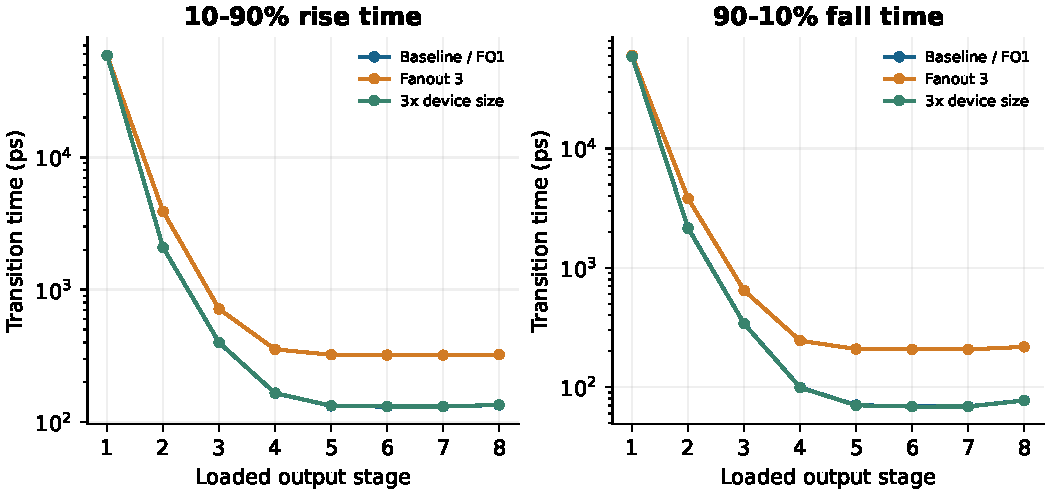
\includegraphics[width=\linewidth]{figures/dic02_stage_evolution.pdf}
\caption{Out1--Out8 rise/fall times under a 2\,$\mu$s input edge, redrawn from actual HSPICE measurement tables, not WaveView screenshots.}
\end{figure}
\begin{figure}[htbp]
\centering
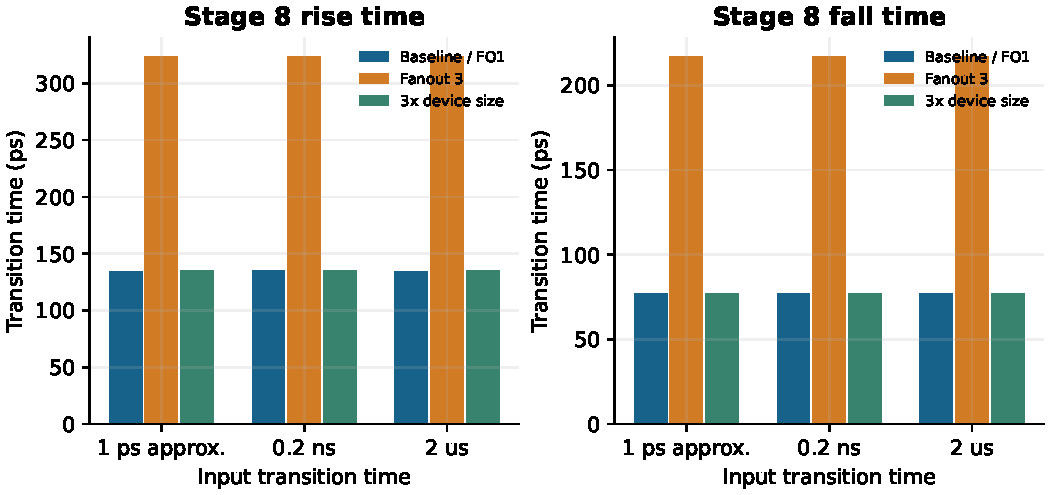
\includegraphics[width=\linewidth]{figures/dic02_stage8.pdf}
\caption{Actual Out8 rise/fall measurements for the three chain configurations and three input edges. Out8 still has a termination-boundary effect; unloaded Out9 is not substituted.}
\end{figure}

For baseline FO1 with a 2\,$\mu$s input edge, Out1 $t_r/t_f$ are 58.881/59.158 ns, Out2 values are 2.081/2.160 ns, and Out3 values are 398.244/340.408 ps. Out6 reaches 130.956/68.551 ps and Out7 reaches 130.927/68.762 ps, showing progressive shaping of the very slow input.

Out8 fall time is approximately 77 ps, compared with about 69 ps at Out7. This is consistent with the boundary loading of the finite nine-stage chain: Out9 has no downstream load, and its output transition affects Out8 through its input capacitance and Miller effect. No separate experiment holding the Out9 load fixed was performed, so this is a mechanism-based explanation rather than an independent causal test. Later stages should not be forced to appear identical. The three initial slews give very similar Out8 results for a given configuration, but rise and fall times are not equal.

The precision check found substantial slow-input early-stage differences with default \texttt{RUNLVL=3}, so those values were not retained. All final cases use \texttt{RUNLVL=6}. For the representative baseline slow-edge chain, the maximum relative difference among all Out1--Out8 rise/fall measurements between \texttt{RUNLVL=5} and 6 is 1.029\%. Out8 rise/fall differences are 0.1175\%/0.0413\%. Changing the near-step from 1 ps to 0.1 ps changes representative Out8 rise/fall by 0.0917\%/0.0124\%. This supports the late-stage conclusions. Early spikes and first-stage details may remain edge-sensitive; the complete exact-zero-edge waveform is not claimed to be reproduced.

\section{Discussion}
Later stages progressively lose sensitivity to the initial input slew and approach a waveform determined by devices and loading. Pull-up and pull-down speeds differ for these dimensions and the supplied model, so $t_r$ and $t_f$ need not be equal.

At a 0.2 ns input edge, FO3 Out8 rise/fall are 323.925/217.054 ps, slower than FO1 at 134.837/77.216 ps. This follows the increased-load trend. The factors need not be exactly three because parasitics, voltage-dependent capacitances and waveforms also change.

With all widths tripled, Out8 is approximately 134.921/76.928 ps, close to baseline. Enlarging every device does not make the full chain three times faster: increased drive is accompanied by increased downstream gate capacitance. This differs from enlarging only the driver while retaining a fixed external capacitance.

Checks cover device count, load connections, all three input conditions, complete Out1--Out8 measurements and representative numerical sensitivity. No original-process numerical values are claimed as achieved. The handout supplies neither a slew tolerance for the supplied model nor a required process corner for this adaptation.

\section{Conclusion}
The nine-stage chain, total-fanout-three chain and enlarged-width chain have all been simulated under all three input-edge conditions. Data show later-stage stabilization, slower FO3 transitions and nearly unchanged slew when driver and load widths are enlarged together. A finite-chain termination effect remains visible. Conclusions apply to the supplied model at 1 V and 25\,$^\circ$C conditions, with the explicit near-step approximation and original-process differences retained.

\end{document}
